\documentclass[12pt]{article}
\usepackage{amsmath}
\usepackage{amssymb}
\usepackage{graphicx}
\usepackage{hyperref}
\usepackage{color}
\begin{document}
\title{A Simple Markov Model Of A Chain With A Single Loop}
\author{Ofir Shukron}
\maketitle
\section{The Model}\label{section_theModel}
In this document we summarize a simple Markov chain describing a chain having N monomers (beads) and one occasion of a loop. Only the first monomer can create a loop with all other $j=2,3,..,N$. We consider bead $N$ to be fixed. 
There are several states for the model. Assuming a loop $[1,j]$, indicating bead 1 is connected to bead $j$, we can form the loops $[1,j+1],[1,j-1]$, or detach, indicated by $[1,0]$. 

Using this terminology, we write\\
$[1,j]\rightarrow [1,j+1] = \lambda$\\
$[1,j]\rightarrow [1,j-1] = \mu$\\
$[1,0]\rightarrow [1,j] = \alpha$\\
$[1,j]\rightarrow [1,0] = \beta$\\
$[1,0]\rightarrow [1,0] = 1-\alpha$\\
where $j=2,3,...,N$
The $\alpha$ value represent the probability of attaching bead 1 to bead $j$ given that there is no loop at time $t$. At first approximation we vary $\alpha$ according to the probability that the beads are closer than some distance, given by the function:
\begin{equation*}
\alpha_{nm}=\Phi(|R_n-R_m|<\epsilon,n-m)=\left[\frac{3}{2\pi b^2|n-m|} \right]^{3/2}\int_0^\epsilon{\exp{\left[-\frac{3k^2}{2|n-m|b^2}\right]dk}}
\end{equation*}
where $b>0$ is the connection length, $R_n$ is the position of bead $n$, and $\epsilon>0$ is the maximal distance in which two beads are considered to have met. 
We indicate the probability to create a loop $[1,j]$ by $p_j$.
Thus, the master equation is given by:
\scriptsize{
\begin{equation*}
\left[\begin{matrix}
\dot{p}_0\\
\dot{p}_2\\
.\\
.\\
.\\
\dot{p_N}
\end{matrix}\right] = 
\left[\begin{matrix}
-N\alpha &\beta             & \beta & ... &... &\beta&\beta\\
\alpha   & -(\beta+\lambda) & \mu   & ... &... &... & 0 \\
\alpha   & \lambda          & -(\beta+\lambda +\mu) &\mu &... &...& 0\\
\alpha   & 0                & \lambda               & -(\beta+\lambda+\mu)&\mu&...& 0\\
.\\
.\\
.\\
\alpha   & 0                & 0 &...& \lambda               & -(\beta+\mu+\lambda)&\mu\\
\alpha   & 0                & 0 &...&  0                    & \lambda & -(\beta+\mu)\\
\end{matrix}\right] 
\left[
\begin{matrix}
p_0\\
p_2\\
.\\
.\\
p_N
\end{matrix}
\right]
\end{equation*}
}
in short notation we write 
\begin{equation*}
\dot{\left[P(t)\right]}=\left[M\right]\left[ P(t)\right]. 
\end{equation*}
the solution to the equation above is given by 
\begin{equation*}
\left[P(t)\right]=\left[P(0)\right]\exp{\left[ Mt\right]}=\left[U\right]exp(\left[D\right]t)\left[U^{-1}\right]\left[P_0\right]
\end{equation*}
where $\left[P(0)\right]$ is the initial distribution of states, $U$ is a matrix of the eigenvectors in its columns, and D is a diagonal matrix with the corresponding  eigenvalues in the diagonal entries.

\section{Simulations}\label{section_simulations}
Setting $\beta=\mu=\lambda=x$ we get 
\begin{equation*}
\left[M\right]=
\left[\begin{matrix}
-N\alpha & x   & x   & ... &... & x & x \\
\alpha   & -2x & x   & ... &... &...& 0 \\
\alpha   & x   & -3x & x   &... &...& 0 \\
\alpha   & 0   & x   & -3x & x  &...& 0 \\
.\\
.\\
.\\
\alpha   & 0   & 0   &...  & x  &-3x& x \\
\alpha   & 0   & 0   &...  &  0 & x &-2x\\
\end{matrix}\right] 
\end{equation*}
choosing $x=1/3$, $d=b/2$, and simulating the system until steady-state (note that $\alpha$ remains as defined above), we find, for a chain of $N=64$ beads that the probability to find a loop $[1,j]$ at steady-state is proportional to $|j-1|$ see Figure \ref{chain64BeadsEqualProbSteadyState} and Figure \ref{loopProbabilitySteadyState64Beads}.

\begin{figure}[h]\label{chain64BeadsEqualProbSteadyState}
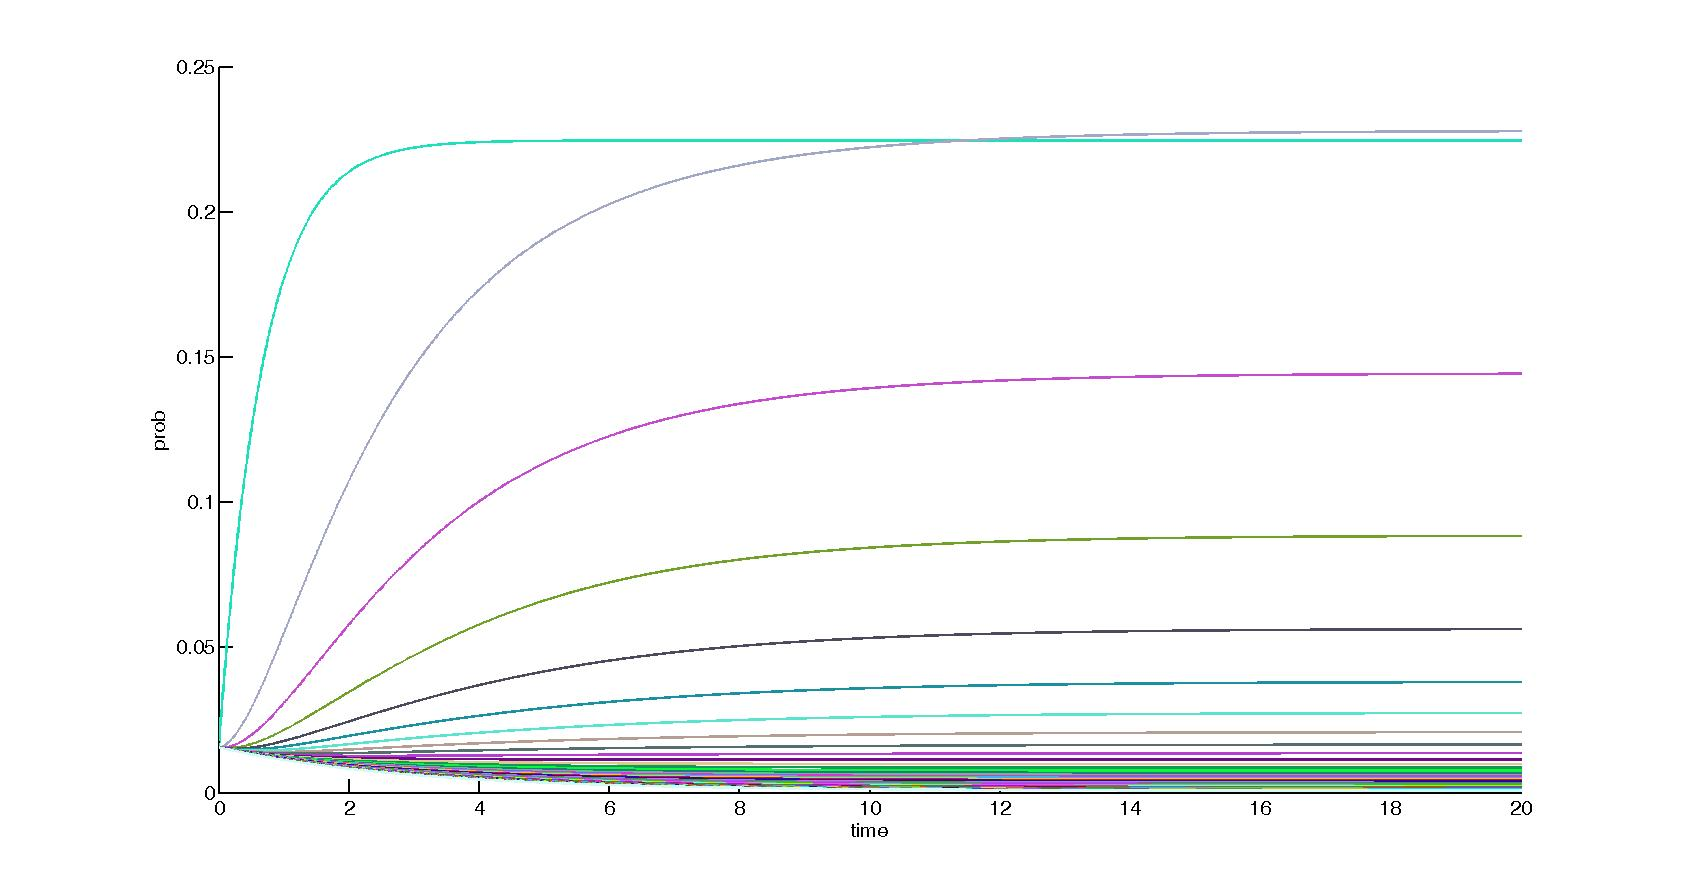
\includegraphics[scale=0.2]{chain64BeadsEqualProbSteadyState}
\caption{\scriptsize{The time evolution of the Markov chain, with $x=1/3$. The values of $\alpha$ remained as defined above. The thick cyan curve represents the probability of no loop. The curves are decreasing (at steady states) with bead number}}
\end{figure}

The steady state probability of loops $[1,j]$ is shown in Figure \ref{loopProbabilitySteadyState64Beads}
\begin{figure}[h]\label{loopProbabilitySteadyState64Beads}
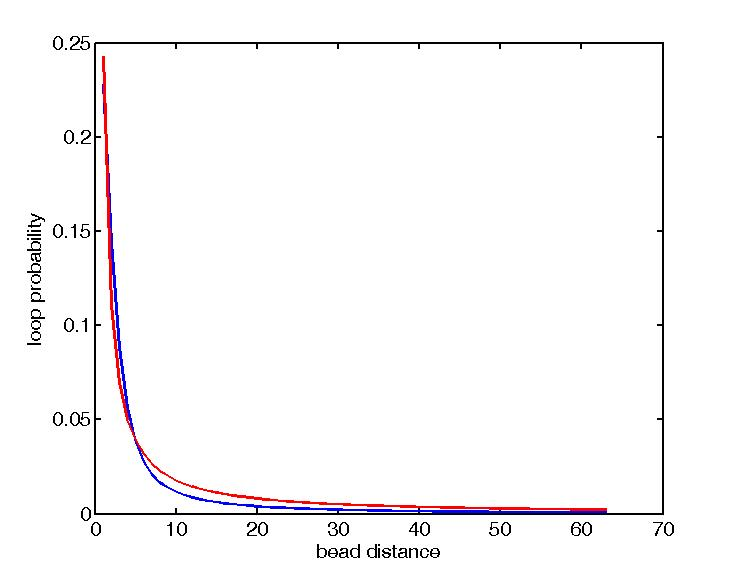
\includegraphics[scale=0.3]{loopProbabilitySteadyState64Beads}
\caption{\scriptsize{The steady state values of the loop probability (blue curve), with $x=1/3$, and $\alpha$ as defined above. To test the theoretical results, that the looping probability is proportional to the bead distance, we fit a model of the kind $y=ax^{-b}$ (red curve). The fitted values are $a=0.2429$, $b=1.137$. The R-square value of the fit is $0.9687$}}
\end{figure}
 
\subsection{Introducing 'hot spots' in the chain} 
We next introduce some beads for which bead 1 have more affinity to, in the sense that once a loop $[1,j]$ is formed,with $j$ being the affine bead to 1, the probability of either detachment $(\beta)$, decreasing ($\mu$) or increasing $(\lambda)$ the loop size are decreased in relation to other beads.

\end{document}